\capitulo{5}{Aspectos relevantes del desarrollo del proyecto}

En este capítulo se explicarán las partes más importantes del desarrollo del proyecto.

\section{Desarrollo de la aplicación web}

Para realizar la primera fase del desarrollo, la recogida de los datos, se ha desarrollado una aplicación web que facilitase las tareas de telerehabilitación conectando al personal especializado con los pacientes con enfermedad de parkinson y que dentro de sus funciones estuviese grabar a los mismos durante la realización de los ejercicios para ser estudiados en tiempo real.

Esta aplicación se ha compuesto de dos partes. Una ha consistido en el diseño y consecuente implementación de una interfaz hombre-máquina fácil de usar y accesible mediante un mando sencillo\footnote{Concretamente un mando de la consola SNES adaptado para ser usado mediante USB}. Esta se compone de una serie de botones de colores, directamente relacionados con los del mando~(figura~\ref{fig:help}), que permiten iniciar una comunicación mediante videoconferencia con el personal terapéutico como finalizar la reunión. Durante el proceso de la llamada, el vídeo del paciente es capturado y enviado al servidor para su procesado posterior.

\begin{figure}
	\centering
	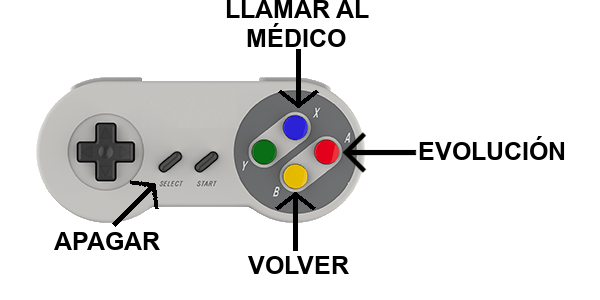
\includegraphics[width=0.7\textwidth]{img/ayuda.png}
	\caption{Funcionalidades del mando de SNES para el control de la aplicación web por parte del paciente.}
	\label{fig:help}
\end{figure}


La segunda parte consiste en la interfaz del terapeuta encargado de dirigir las sesiones de rehabilitación del paciente ofreciendo una interfaz sencilla que permite conectarse a las videoconferencias de los diferentes pacientes y dirigir las sesiones de terapia además de gestionar la evolución del paciente~(figura~\ref{fig:menu_respon}).

\begin{figure}
	\centering
	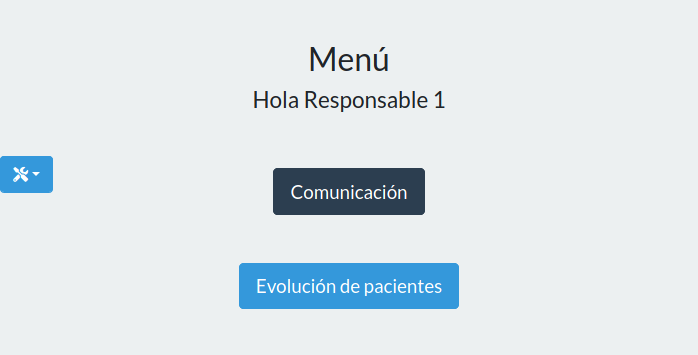
\includegraphics[width=0.8\textwidth]{img/menu_responsable.png}
	\caption{Menú del terapeuta}
	\label{fig:menu_respon}
\end{figure}

Las características del equipo donde está desplegada la aplicación del paciente es:
\begin{itemize}
	\item MSI - Cubi N 8GL-001BEU N4000 1.10GHz.
	\item WB Green M.2 120 GB SATA 3.
	\item X GB DDR4 2400 MHz.
	\item Lubuntu x86\_64 18.04.
	\item WebCam Logitech HD Pro C920
\end{itemize}

TODO: Quizás sería interesante explicar las valoraciones otorgadas de la aplicación si se tienen antes de la entrega del trabajo. 
